\documentclass[letterpaper,12pt]{article}
\usepackage[justification=centering]{caption}
\usepackage{float}
\usepackage[usenames,dvipsnames]{color}
\usepackage{subfigure}
\usepackage[margin=2.1cm]{geometry}
\usepackage{changepage}
\usepackage{titlesec}
\usepackage{tcolorbox}
\usepackage[affil-it]{authblk} 
\usepackage{etoolbox}
\usepackage{lmodern}
\usepackage{amsmath}
\usepackage{amssymb}
\usepackage{mathrsfs}
\usepackage{mathtools}
\usepackage{bbm}
\usepackage{MnSymbol}
\usepackage{hyperref}
\hypersetup{
	colorlinks=true,
	linkcolor=blue,
	filecolor=magenta,      
	urlcolor=cyan,
	citecolor = blue,
}

\newtheorem{prop}{Proposition}[section]
\newtheorem{corollary}{Corollary}
\newtheorem{assumption}{Assumption}
\newtheorem{defi}[prop]{Definition}
\newtheorem{theorem}{Theorem}
\newtheorem{algorithm}{Algorithm}
\newtheorem{remark}[prop]{Remark}
\newtheorem{exam}[prop]{Example}
\newtheorem{lemma}{Lemma}
\newcommand{\VXb}{VIX }

% Bibliography preamble
\usepackage[numbers,sort&compress]{natbib}

\makeatletter
\patchcmd{\@maketitle}{\LARGE \@title}{\fontsize{22}{20}\selectfont\@title}{}{}
\makeatother
\renewcommand\Authfont{\fontsize{12}{14.4}\selectfont}
\captionsetup{margin=18pt,format=hang,justification=justified}
\marginparsep 20pt
\marginparwidth 50pt 

\begin{document} 
	\title{Recurrent Neural Network}
	\author{Congshan Zhang}
	\date{}
	\maketitle
\section{Unfolding a Recurrent Neural Network}
The training set $X$ contains $N$ individuals and $D$ features over $T$ periods. So we can represent it as a three-dimensional tensor with shape $(N\times T\times D)$.

We have an unfolded RNN below in Figure \ref{fig:rnn}.
\begin{figure}[H]
	\begin{center}
		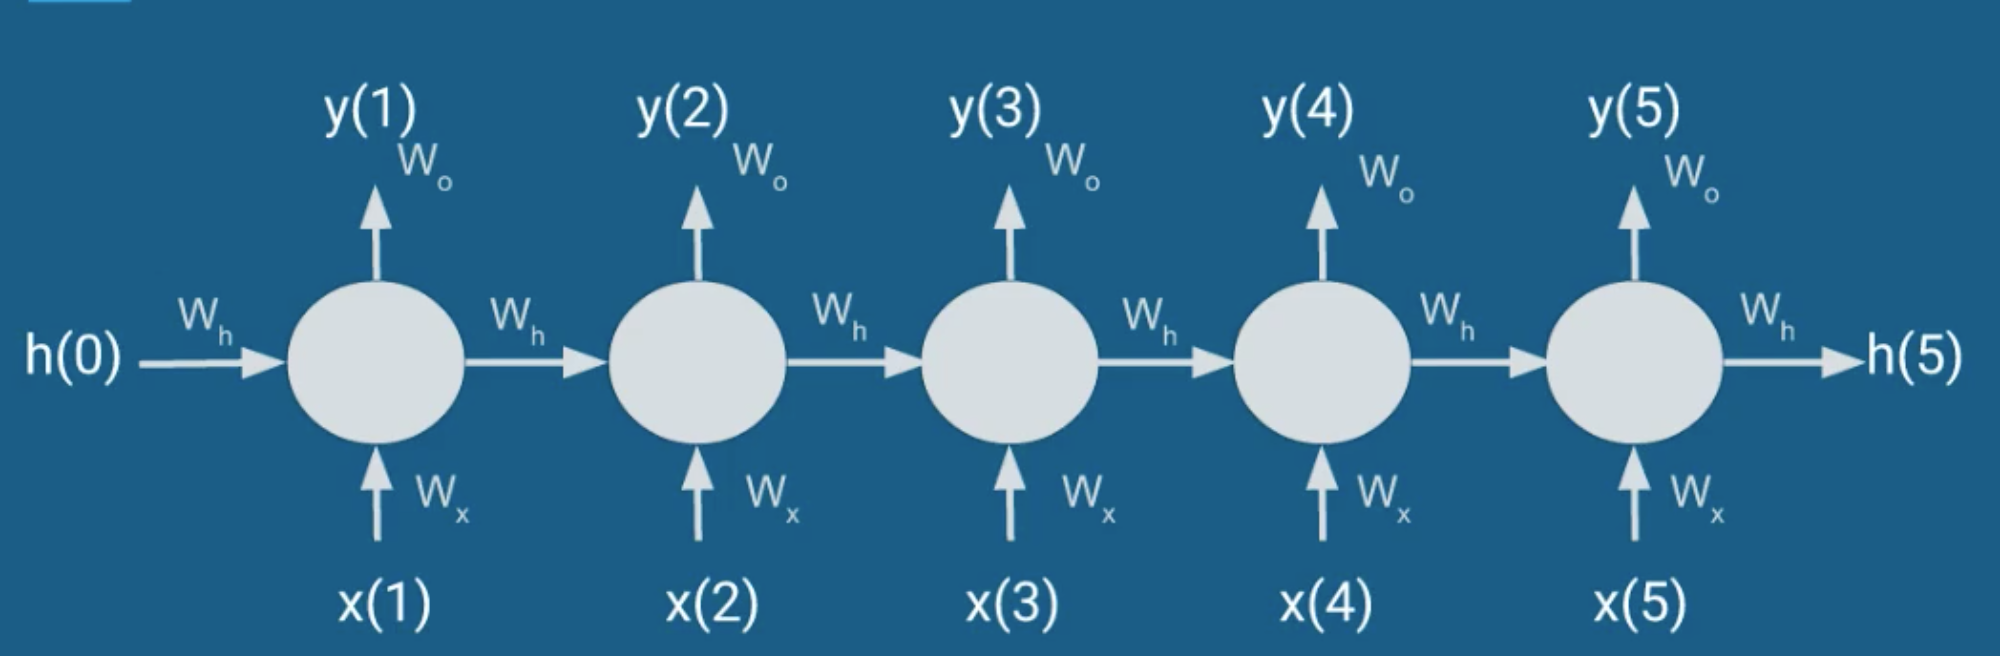
\includegraphics[width=10cm,clip]{rnn.png}
	\end{center}
	\caption{This is an illustration of a recurrent neural network with shared weighting.}\label{fig:rnn}
\end{figure}

\subsection{Backpropagation Through Time (BPTT)}

At time $t$, the output of the network is 
\begin{align}
\hat{y}(t) = softmax\left(W_o^Th(t)\right).
\end{align}
Applying the definition of $h(t)$ yields
\begin{align}
\hat{y}(t) = softmax\left(W_o^T f\left( W_h^T h(t-1) + W_x^Tx(t) \right)\right).
\end{align}
One can write it recursively as
\begin{align}
\hat{y}(t) &= softmax\left(W_o^T f\left( W_h^T f\left(W_h^T h(t-2) + W_x^Tx(t-1)\right) + W_x^Tx(t) \right)\right)\nonumber\\
& = \cdots\cdots
\end{align}




\clearpage
\bibliographystyle{chicago}
\bibliography{rnn.bib}


\end{document}